\RequirePackage{tikz}
\documentclass{article}
\usepackage[colorlinks=true,citecolor=blue]{hyperref}
\usepackage[T1]{fontenc}
\usepackage{tikz}
\usepackage{pgfplots}
\usetikzlibrary{shapes,positioning,calc,arrows.meta,arrows,patterns,patterns.meta,fit}
\usepackage{tikzscale}
\usepackage{amsmath,bm}
\usepackage{amssymb}

\begin{document}

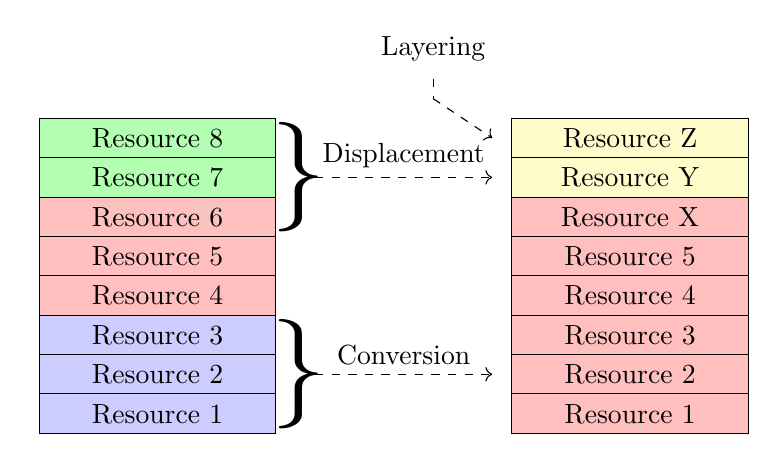
\begin{tikzpicture}
% First Stack
\foreach \i in {1,2,3}
    \draw [fill=blue!20] (0,{(\i-1)*0.5}) rectangle (3,{\i*0.5}) node[pos=.5] (res\i) {Resource \i};

\foreach \i in {4,5}
    \draw [fill=red!25] (0,{(\i-1)*0.5}) rectangle (3,{\i*0.5}) node[pos=.5] (res\i) {Resource \i};

\foreach \i in {6}
    \draw [preaction={fill=green!30},pattern={Lines[angle=-45, line width=3mm]}, pattern color=red!25] (0,{(\i-1)*0.5}) rectangle (3,{\i*0.5}) node[pos=.5] (res6) {Resource \i};


\foreach \i in {7,8}
    \draw [fill=green!30] (0,{(\i-1)*0.5}) rectangle (3,{\i*0.5}) node[pos=.5] (res\i) {Resource \i};


% Arrow between stacks
\draw [->, dashed] (3.5,0.75) -- (5.75,0.75) node[midway, above] {Conversion};
\draw [->, dashed] (3.5,3.25) -- (5.75,3.25) node[midway, above] {Displacement};

\node [fit=(res1) (res2) (res3)] (fitblue) {};
\path let \p1=(fitblue.north west), \p2 = (fitblue.south west) in
   node [right of=fitblue, xshift=2.25em] {%
   \pgfmathsetmacro\heightoffit{.6*(\y1-\y2)}%
   \resizebox{!}{\heightoffit pt}{\}}%
 };

\node [fit=(res6) (res7) (res8)] (fitgreen) {};
\path let \p1=(fitgreen.north west), \p2 = (fitgreen.south west) in
   node [right of=fitgreen, xshift=2.25em] {%
   \pgfmathsetmacro\heightoffit{.6*(\y1-\y2)}%
   \resizebox{!}{\heightoffit pt}{\}}%
 };


\draw [-, dashed] (5,{8.5*0.5+0.25}) -- (5,{8.5*0.5}) node[above,yshift=10] {Layering};


\draw [->, dashed] (5,{8.5*0.5}) -- (5.75,{7.5*0.5});

% Second Stack


\foreach \i in {1,2,3,4,5}
    \draw [fill=red!25] (6,{(\i-1)*0.5}) rectangle (9,{\i*0.5}) node[pos=.5] {Resource \i};

\draw [fill=red!25] (6,{(6-1)*0.5}) rectangle (9,{6*0.5}) node[pos=.5] {Resource X};

\draw [fill=yellow!20] (6,{(7-1)*0.5}) rectangle (9,{7*0.5}) node[pos=.5] {Resource Y};

\draw [fill=yellow!20] (6,{(8-1)*0.5}) rectangle (9,{8*0.5}) node[pos=.5] {Resource Z};




\end{tikzpicture}

\end{document}